\documentclass[a4paper,10pt]{article}

\usepackage[latin1]{inputenc}
\usepackage[portuges]{babel}
\usepackage[pdftex]{graphics,color}
\usepackage[pdftex]{graphicx}
\usepackage{wrapfig} 
\usepackage{epsfig} 
\usepackage{url}
\usepackage{ae,algorithm,alltt}
\usepackage{amsfonts,amstext,enumerate}
\usepackage{float,fancyvrb,fontenc}
\usepackage{geometry,hyperref,ifthen}
\usepackage{indentfirst,lastpage,longtable}
\usepackage{lscape,makeidx,mathrsfs}
\usepackage{multicol,pifont,psfrag}
\usepackage{setspace,showidx,subfigure}
\usepackage{texnames,textcomp,ulem}
\usepackage{url,varioref,version}
\usepackage{wasysym}

\begin{document}

\pagestyle{myheadings}
\markboth{}{\rm Lentes e polariza��o da luz}
\renewcommand{\thefootnote}{\fnsymbol{footnote}}	

\title {Lentes e Polariza��o da luz}  
\author {I.R. Pagnossin \\ irpagnossin@hotmail.com \and R.B. Naca \\ rogerio\_naca@procomp.com.br}
\date {\today}
\maketitle

\begin{abstract}
  	No presente experimento procuramos evidenciar v�rias leis utilizadas na �ptica geom�trica e
�ptica f�sica. Come�amos por verificar a {\it lei dos pontos conjugados} determinando, para isso,
a dist�ncia focal de uma lente convergente. Em seguida comparamos duas formas diferentes de se calcular 
a {\it amplifica��o linear} desta mesma lente: $m=-i/o$ e $m=h_i/h_o$. A lente divergente, que n�o forma 
imagem
projet�vel, tornou-se um bom exerc�cio no que tange as conven��es ``estranhas'' utilizadas pela �ptica
geom�trica durante a determina��o indireta de sua dist�ncia focal. A lupa, outro instrumento bastante
�til e conhecido foi tamb�m avaliado. Mais interessante ainda foi o estudo do ``efeito lupa'' que um orif�cio
pequeno assume. Em seguida, e j� passando para a �ptica f�sica, estudamos a polariza��o de um laser de
He--Ne, o {\it �ngulo de Brewster} e sua rela��o com o {\it �ndice de refra��o}, 
{\it coeficientes de reflex�o} e a {\it Lei de Malus}. Finalmente,
divertimo-nos com o interessante efeito da {\it birrefring�ncia} e {\it fotoelasticidade}.
 
\end{abstract}
\section{Introdu��o te�rica} 
  	Os conceitos te�ricos aqui envolvidos englobam duas experi�ncias: Lentes e polariza��o da luz. 
Temos em mente associar todos os conceitos de forma a ambas as experi�ncias se complementarem.\footnote{Esta
introdu��o te�rica baseia-se principalmente no trabalho \cite[p�g.4]{alex}.} 

	Lente esf�rica � um sistema �ptico onde predomina a refra��o e possui pelo menos um dioptro (fronteira que
divide dois meios) esf�rico. Os raios das esferas que originam as faces das lentes s�o chamados {\it raios de curvatura}.
Quando uma das faces � plana, admitios que seu raio de curvatura � infinito. Quando os raios de curvatura s�o id�nticos,
a lente � dita {\it sim�trica} (Biconcava ou biconvexa). As leis aqui introduzidas levar�o em conta as condi��es de nitidez
de Gauss que, mais especificamente, determina que as lentes devem ser delgadas, ou seja, que sua espessura 
deve ser muito pequena 
quando comparada com os raios de curvatura, e que os raios que nas lentes chegam sejam paraxiais. Segue abaixo a figura
 1 onde vemos os seis tipos de lentes esf�ricas poss�veis, apresentando na primeira linha lentes de
bordas finas (convergentes) e na segunda, lentes de bordas grossas (divergentes).

%\begin{figure}[H]
  %\centering
  %\includegraphics[scale=0.5]{figuras/exercicio1.jpg}
  %\label{fig:exercicio 1} 
  %\caption{\footnotesize Os seis tipos poss�veis de lentes esf�ricas.}
%\end{figure} 



	Quanto � nomenclatura, enunciamos primeiramente a face de menor raio de curvatura ao nome da lente. Uma importante 
rela��o matem�tica � a chamada {\it equa��o do fabricante} para lentes delgadas esf�ricas, onde relaciona a abscissa
focal de uma lente delgada (ou dist�ncia focal), e pode ser expressa atrav�s de:
	$$
	{1\over f}=(n-1)[{1\over R_1}-{1\over R_2}]+{(n-1)^2\over n}{t\over R_1R_2}
	$$
	
	onde $n$ � o �ndice de refra��o, $R_1$ e $R_2$ s�o os raios de curvatura das respectivas lentes e $t$ a espessura
das mesmas. Quando a face � convexa, associamos um valor positivo ao raio. Ou seja, o raio de curvatura $R_1$ ou $R_2$ �
positivo se o centro de curvatura est� do lado real. Quando o centro de curvatura estiver do lado virtual, o raio ser�
negativo (face c�ncava). Uma lente � chamada convergente quando a dist�ncia focal $f$ � positiva e divergente para $f$
negativa. 


	Vejamos mais detalhadamente a figura 1: As lentes na perte de cima s�o convergentes e, 
portanto, todas tem $f>0$. As de baixo s�o divergentes e, por conseguinte, $f<0$. Da esquerda para a direita
temos $R_1<0$ e $R_2>0$; $R_1<0$ e $R_2=+\infty>0$; $R_1,R_2<0$; $R_1<0$ e $R_2>0$; $R_1=-\infty<0$ e
$R_2>0$; $R_1,R_2>0$.  

	Para que uma imagem possa ser completamente caracterizada, devemos conhecer sua natureza e posi��o. Quanto �
natureza, podemos classificar uma imagem em real, virtual ou impr�pria e, com rela��o � posi��o, devemos conhecer os
elementos que nos permitam localizar a imagem em rela��o ao sistema �ptico. Um ponto � classificado �pticamente como
ponto objeto quando � o v�rtice de um pincel de luz incidente em um sistema �ptico. H� tr�s tipos poss�veis na fam�lia
{\it objeto}:

\begin{description}
\item [Ponto Objeto Impr�prio:] � v�rtice de um pincel incidente de formato cil�ndrico.
\item [Ponto Objeto Real:] � v�rtice de um pincel incidente de formato c�nico divergente.
\item [Ponto Objeto Virtual:] � v�rtice de um pincel incidente de formato c�nico convergente.
\end{description}

	Um ponto � considerado ponto imagem quando � o v�rtice de um pincel de luz emergente de um sistema �ptico. H�
tr�s tipos poss�veis na fam�lia {\it imagem}:

\begin{description}
\item [Ponto Imagem Impr�prio:] � v�rtice de um pincel emergente de formato cil�ndrico.
\item [Ponto Imagem Real:] Uma imagem � dita real quando os raios luminosos passam ou podem passar pela imagem, ou seja,
	� um v�rtice de um pincel emergente de formato c�nico convergente.
\item [Ponto Imagem Virtual:] Um ponto � classificado opticamente como virtutal quando a imagem se forma no prolongamento
	dos raios luminosos. Ou seja, quando � v�rtice de um pincel emergente c�nico divergente.
\end{description}

	A dist�ncia $i$ que define a posi��o da imagem ser� positiva quando a imagem estiver do lado real; Mas a 
dist�ncia $o$ que localiza o objeto ser� positiva quando estiver do lado virtual e negativa caso esteja no outro lado.

	As posi��es $o$ do objeto e $i$ da imagem, na aproxima��o de raios paraxiais, relacionam-se pela {\it equa��o
dos pontos conjugados} ou {\it equa��o de Gauss} para lentes:
	$$
	{1\over f}={1\over i}+{1\over o}
	$$
	
	A amplifica��o linear transversal da imagem � definida como a raz�o entre as alturas da imagem e do objeto:
	$$
	m={h_i\over h_o}
	$$

	Observando a figura 2 e notando que os tri�ngulos
$\Delta ABC$ e $\Delta DEC$ s�o 
 semelhantes, fica claro que 
 	$$
	{h_i\over h_o}={i\over o}
	$$

	que � a chamada {\it equa��o de amplifica��o linear transversal}, exceto pelo sinal negativo acrescentado por
quest�o das normas aqui introduzidas:
	$$
	m=-{i\over o}
	$$

	onde uma amplifica��o linear negativa significa uma imagem invertida.

%\begin{figure}[htb]
  %\centering
  %\includegraphics[scale=0.5]{figuras/exercicio2.jpg}
  %\label{fig:exercicio 2}
  %\caption{\footnotesize Dedu��o da lei de amplifica��o linear transversal para lentes.}
%\end{figure} 

	O �ngulo de vis�o do objeto com a lupa � dado por
	$$
	\theta \cong -{h_i\over i}={h_o(-i/o)\over -i}={h_o\over o}=h_o({1\over f}-{1\over i})
	$$

	J� a amplifica��o angular de um instrumento �ptico pode ser definida como a raz�o entre o �ngulo de vis�o de um
objeto com o instrumento e o �ngulo de vis�o do mesmo a olho nu. Matematicamente escrevemos
	$$
	M={\theta\over\theta_p}\cong{L_p\over f}-{L_p\over i}
	$$

	� bom ressaltar que a dist�ncia $i$ depende da acomoda��o do olho. A m�xima amplifica��o angular da lupa ser�
dada quando $i$ for negativo e tiver o menor m�dulo poss�vel. Ou seja, para $i=-L_p$. Com isso teremos
	$$
	M_L={L_p\over f}+1
	$$

	mas, na pr�tica, para uma vis�o relaxada, a imagem se forma a uma grande dist�ncia (infinito) pois, em geral, 
mediante esta situa��o, pode-se considerar o objeto no foco da lupa e � por isso que a equa��o abaixo � considerada como
a amplifica��o angular da lupa:
	$$
	M_L={L_p\over f}
	$$

	Se acoplarmos duas lentes justapostas de dist�ncias focais $f_1$ e $f_2$ separadas por uma dist�ncia $D$ muito pequena,
as mesmas se comportam como uma �nica lente de dist�ncia focal $f$ dada por
	$$
	{1\over f}={1\over f_1}+{1\over f_2}-{1\over f_1f_2}
	$$

	Mesmo levando em conta todos os cuidados para que as aproxima��es sejam o mais realistas quanto o poss�vel, ainda 
h� possibilidades para que a imagem formada pela lente apresente certas ``aberra��es crom�ticas''. Este fen�meno acontece
pois a dist�ncia focal depende do �ndice de refra��o e este do comprimento de onda da luz, com isso formando imagens em
posi��es diferentes para cores diferentes. Podemos corrigir satisfat�riamente este problema se utilizarmos duas lentes
justapostas cada uma com um �ndice de refra��o e uma sendo divergente e a aoutra convergente. A este arranjo d�-se o nome
de {\it dupleto acrom�tico}. Outro grande problema, a aberra��o esf�rica, � causada por uma lente simples com uma superf�cie
esf�rica que n�o gera uma imagem puntiforme de um objeto puntiforme. H� ainda outras aberra��es ligadas �s distor��es na
imagem de um objeto extenso chamadas {\it astigmatismo} e {\it coma}.

	Dando in�cio � discuss�o sobre os conceitos te�ricos da segunda parte de nossa experi�ncia, come�aremos por definir
uma onda linearmente polarizada. 

	A dire��o do campo el�trico de uma onda eletromagn�tica, ou seja, o vetor campo el�trico, do vetor de Poyting, 
define o estado de polariza��o da luz. Entende-se por polariza��o linear o fato de o vetor campo el�trico estar sempre
paralelo a um plano definido (Plano de polariza��o da onda). A figura 3  mostra-nos uma onda
plano polarizada ou polarizada linearmente no plano $xy$.

%\begin{figure}[htb]
  %\centering
  %\includegraphics[scale=0.5]{figuras/ondaeletromagetica.jpg}
  %\label{fig:onda eletromagn�tica}
  %\caption{\footnotesize Onda plano--polarizada}
%\end{figure}

	Como vimos na figura 3, o campo el�trico pode ser escrito como 
	$$
	\mathbf{E}(x,t)=E_0\cos(kx-\omega t)\hat j
	$$

	onde $k$ � o n�mero de onda angular definido matematicamente por $k=2\pi/\lambda$ e $\omega$ � a freq��ncia
angular.

	Para uma dada posi��o fixa em $x$ o campo el�trico realiza uma oscila��o harm�nica com freq��ncia angular
$\omega$ e, num dado instante $t$ fixo, o campo el�trico varia harmonicamente com a posi��o $x$. A onda eletromagn�tica
� chamada circularmente polarizada quando o campo el�trico gira em torno da dire��o de propara��o, possuindo m�dulo
constante. Analogamente, quando o vetor campo el�trico descreve uma el�pse, a onda � chamada elipticamente polarizada.
Sabemos que, matematicamente, a onda elipticamente polarizada pode ser descrita como a superposi��o de duas ondas 
linearmente polarizadas em dire��es perpendiculares e defasadas de $90^{\mathrm{o}}$. Particularmente, este tipo de
superposi��o e com ondas de mesma amplitude resulta numa onda circularmente polarizada. � de relativa import�ncia que a
superposi��o de duas ondas ortogonais linearmente polarizadas e em fase resulta numa nova onda linearmente polarizada.

	Num espa�o livre, a onda elipticamente polarizada � o estado mais geral de polaria��o definida. Facilmente podemos
perceber que a defini��o de onda n�o polarizada resulta de uma polariza��o que varia rapidamente e de maneira completamente
aleat�ria no tempo. H� ainda alguns casos h�bridos onde certo tipo de radia��o pode ter sua polariaza��o variando lentamente
no tempo ou ainda a radia��o ser parcialmente polarizada, que � a superposi��o de uma radia��o de polariza��o definida com
uma n�o polarizada.

	A luz n�o polarizada � usualmente representada como uma superposi��o de ondas polarizadas ortogonais. Observe 
abaixo o exemplo de um feixe de luz n�o polarizada incidente numa superf�cie:

%\begin{figure}[htb]
  %\centering
  %\includegraphics[scale=0.5]{figuras/naopolarizada.jpg}
  %\caption{\footnotesize Reflex�o de luz n�o polarizada num meio material transparente. O feixe refletido � parcialmente
	%polarizado.}
%\end{figure}

	Perceba que este feixe representado na figura acima apresenta uma polariza��o paralela ao plano de incid�ncia e
tamb�m uma polariza��o perpendicular a este plano. Pelo fato desta superposi��o apresentar um car�ter aleat�rio das fases
envolvidas, este n�o � um caso de polariza��o definida.

	H� v�rios m�todos para se obter uma onda eletromagn�tica linearmente polarizada a partir de uma onda n�o polarizada. Esses m�todos baseiam-se em diferentes propriedades dos estados ortogonais de polariza��o, como por exemplo, 
diferentes atenua��es (dicro�smo), diferentes �ndices de refra��o, diferentes propriedades de reflex�o, telas de fios
paralelos para radia��o infravermelha distante, cristais birrefringentes, prismas especiais, etc.

	Um conceito importante que surge neste ponto � o de �ngulo de Brewster, que � o �ngulo de incid�ncia
caracter�stico de um material no qual um feixe de luz n�o polarizado incidente � refletido polarizadamente
no plano de incid�ncia (Perpendicular ao dioptro). Este �ngulo caracteriza-se pela igualdade 
\cite[p�g.390]{griffiths}
	$$
	{\cos\theta_T\over\cos\theta_I}={\mu_1 n_2\over\mu_2 n_1}=\beta
	$$

	onde $\theta_T$ � o �ngulo de emerg�ncia do raio refratado, $\theta_I$ o �ngulo de incid�ncia do
feixe n�o polarizado, $\mu_1$ e $\mu_2$ s�o as permeabilidades magn�ticas nos meios $1$ (origem) e $2$
(destino) de �ndices de refra��o $n_1$ e $n_2$, respectivamente. Ent�o
\begin{eqnarray*}
{\sqrt{1-\sin^2\theta_T}\over\cos\theta_I}	&=& \beta			\\
\sqrt{1-\sin^2\theta_T}				&=& \beta\cos\theta_I		\\
1-\sin^2\theta_T				&=& \beta^2\cos^2\theta_I	\\
1-({n_1\over n_2})^2\sin^2\theta_I		&=& \beta^2\cos^2\theta_I	\\
						&=& \beta^2(1-\sin^2\theta_I)	\\
						&=& \beta^2-\beta^2\sin^2\theta_I	\\
1-\beta^2					&=& [({n_1\over n_2})^2-\beta^2]\sin^2\theta_I	
\end{eqnarray*}

	Tomando $\mu_1\cong\mu_2$, que � uma aproxima��o quase sempre poss�vel,
\begin{eqnarray*}
1-\beta^2				&=& [{1\over\beta^2}-\beta^2]\sin^2\theta_I		\\
\sin^2\theta_I				&=& {\beta^2(1-\beta^2)\over(1-\beta^4)}		\\
					&=& {\beta^2\over1+\beta^2}				\\
\sin^2\theta_I+\beta^2\sin^2\theta_I	&=& \beta^2						\\
\beta^2\cos^2\theta_I			&=& \sin^2\theta_I					\\
\tan^2\theta_I				&=& \beta^2						\\
\tan\theta_I				&=& {n_2\over n_1}			
\end{eqnarray*}

	Nesta situa��o, o �ngulo de incidncia $\theta_I$ � conhecido como o �ngulo de Brewster $\theta_B$ e,
assumindo $n_1=1$, resulta que
	$$
	\tan\theta_B\cong n_2
	$$
	 
	Um exemplo de aplica��o do �ngulo de Brewster s�o os �culos de Sol com lentes polar�ides, que
reduzem os reflexos luminosos de superf�cies tais como �gua, pisos, etc. O que estes �culos fazem �
polarizar a luz incidente no plano paralelo � superf�cie refletora. Mas, como acabamos de ver,
n�o existe componente paralela a esta superf�cie quando a luz incide no �ngulo de Brewster. O resultado,
ent�o, � o anulamento quase total da luz oriunda dessas superf�cies.

	Falaremos agora sobre uma importante lei, a de Malus. Um polarizador ideal deixa transmitir toda uma determinada
polariza��o e elimina perfeitamente a outra. Mostraremos abaixo um esbo�o de onda incidente na dire��o $\hat i$, com vetor
campo el�trico tendo componentes $E_y$ e $E_z$. Se um polarizador $P1$ estiver alinhado na dire��o $y$, somente a componente
$E_y$ do campo ser� transmitida. E, se um polarizador $P2$ estiver formando um �ngulo $\theta$ com $P1$, somente a componente
$E_t$ do campo el�trico ser� transmitida. De outra forma,
	$$
	E_t=E_y\cos\theta
	$$

	Uma vez que a intensidade da onda � proporcional ao quadrado da amplitude, resulta em intensidade transmitida pelo
polarizador ideal $P2$:
	$$
	I_t=I_0\cos^2\theta
	$$

	Esta equa��o traduz matematicamente o resultado da lei de Malus. Se existir uma luminosidade ambiente que n�o vem
do polar�ide, e que esta fra��o de polariza��o indesejada seja transmitida ao polar�ide, a lei de Malus pode ser reescrita
na forma
	$$
	I_t=I_0\cos^2\theta+I_f
	$$
	
	onde $I_0$ � a intensidade m�xima e $I_f$ a intensidade m�nima quando
$\theta=90^{\mathrm{o}}$.

	Mas os polar�ides n�o s�o ideais e absorvem intensidade luminosa mesmo quando posicionados de forma
favor�vel � luz incidente. Isto pode tamb�m pode ser percebido nos �culos de Sol, que reduzem em cerca de
$1/4$ a intensidade da luminosidade natural justamente por este motivo.

	Vejamos um exemplo de aplica��o da Lei de Malus: Tome um conjunto de $10$ polarizadores ideais
alinhados a uma fonte n�o polarizada de intensidade $I_0$, de forma que cada polarizador forma um �ngulo de
$10^{\mathrm{o}}$ em rela��o ao anterior. Qual a fra��o da intensidade do feixe que sai do �ltimo 
polar�ide? Ap�s o primeio polar�ide a intensidade $I_1$ observada ser�
	$$
	I_1=I_0\cos^2\theta
	$$

	sendo $\theta=10^{\mathrm{o}}$. Agora, no segundo polar�ide incide uma intensidade $I_1$ e,
consequentemente, enxergamos
	$$
	I_2=I_1\cos^2\theta=I_0\cos^2\theta\cos^2\theta
	$$

	e assim sucessivamente at� o d�cimo polarizador:
	\begin{eqnarray*}
	I_{10}=I_9\cos^2\theta	&=& I_0\cos^{20}\theta	\\
			   	&=& 0,0563\cdot I_0
	\end{eqnarray*}

	Ou seja, apenas $5,6\%$ da intensidade inicial emerge do �ltimo polarizador.













\section{An�lise de dados} 
  \subsection{Lentes convergentes}\label{sec:lc} 
    	Primeiramente verificamos a lei dos pontos conjugados ao determinar a dist�ncia focal de uma
lente convergente. Al�m disso, tamb�m foi poss�vel verificar a veracidade da equa��o de amplifica��o
linear $m=-i/o$. Para isso posicionamos uma fonte luminosa, uma lente convergente e um anteparo 
opaco tal como demonstrado na figura 5.

%\begin{figure}[htb]
  %\centering
  %\label{fig:lente convergente}
  %\includegraphics[scale=0.25]{figuras/Alc.jpg}
  %\caption{\footnotesize Arranjo experimental que possibilitou a verifica��o da lei dos pontos conjugados
%e a express�o da amplifica��o linear: O objeto, representado por uma fonte luminosa na forma de uma cruz
%de malta de dimens�es $2,35\,\mathrm{cm}\times1,65\,\mathrm{cm}$ � captado pela lente convergente ($C36$)
%que projeta a imagem real sobre o anteparo mais a frente. A posi��o de forma��o da imagem � identificada 
%como aquela em que a imagem forma-se em foco.}
%\end{figure} 

	Note que este procedimento s� � poss�vel por que lentes convergentes formam imagens reais, poss�veis
de se projetar. De fato, veremos mais a frente (sess�o \ref{sec:ld}) que no caso de lentes
divergentes a situa��o complica-se quando queremos determinar sua dist�ncia focal.

	Mantemos, ent�o, a fonte fixa e variamos as posi��es da lente e do anteparo (ou, equivalentemente,
do objeto e da imagem, respectivamente) e medimos estas posi��es mais o tamanho vertical\footnote{Tamb�m 
poder�amos ter medido a 
dimens�o horizontal mas, devido �s posi��es dos objetos sobre a bancada, esta medida mostrou-se ser 
desajeitadamente dif�cil de se conseguir.} da imagem formada. Isto posto � f�cil encontrar os conjuntos
$(i,\sigma_i)$ e $(h_i,\sigma_{h_i})$, cujas incertezas foram avaliadas em $0,5\,\mathrm{mm}$. J� para o
grupo $(o,\sigma_o)$ procedemos da seguinte forma: Procuramos posicionar o anteparo uma vez se aproximando
da lente e outra se afastando. Com isso determinamos as posi��es m�xima e m�nima para a forma��o em foco,
conforme nossa avalia��o fisiol�gica, da imagem. Da� obtemos a m�dia ($o$) e o desvio padr�o; a este 
�ltimo somamos quadraticamente a incerteza sistem�tica $0,5\,\mathrm{mm}$ utilizada para os conjuntos 
anteriores de modo a obter $\sigma_o$. O passo seguinte foi inverter $o$ e $i$ de modo a linearizar a
equa��o de Gauss:
	$$
	{1\over i} = {1\over f} - {1\over o} \Rightarrow y = {1\over f} - x
	$$

	O c�lculo de incertezas mostra que $\sigma_y=y^2\sigma_i$, valendo o mesmo para $x$. Plota-se
o gr�fico $1/i\times 1/o$, faz-se a transfer�ncia de incertezas 
	$$
	\sigma_y^2=\sigma_{y_0}^2+m^2\sigma_x^2
	$$ 

	e refazemos o gr�fico de forma mais precisa: $(y,\sigma_y)\times x$ e ajusta-se a reta. Obtivemos
$y=0,03977(2)-0,999(15)\,x$, dando-nos 
	$$
	f = {1\over 0,03977} = 25,14(13)\,\mathrm{cm\,,}
	$$ 

	sendo a incerteza encontrada simplesmente por
	$$
	\sigma_f = f^2\sigma_a = 25,145^2 \times 0,0002 = 0,13
	$$

	onde $f$ � obviamente a dist�ncia focal (em cent�metros) e $a$ � apenas o coeficiente linear
da curva ajustada. Note que, al�m da incerteza para nos dar uma no��o de acur�cia, o coeficiente
angular comporta-se como o previsto, pois � muito pr�ximo da unidade; �, de fato, indistingu�vel,
dada a sua incerteza.  
	
	Uma forma de avaliar se o resultado obtido est� correto � tentar focalizar um objeto muito
dist�nte. Neste caso, a imagem formar-se-� justamente no foco:
	$$
	\lim_{o\rightarrow\infty} {1\over f} = \lim_{o\rightarrow\infty} {1\over i}+{1\over o} = {1\over i}
		\Rightarrow i=f
	$$

	Utilizamos como objeto distante o Sol e encontramos $f=25,0\pm 2,0\,\mathrm{cm}$. A incerteza aqui �
bastante grande pois a medida era desajeitada de se conseguir. De qualquer modo vemos que de fato h�
coer�ncia entre os resultados\footnote{Apenas como complemento da informa��o, medimos tamb�m a dist�ncia
focal da lente $C5$ pelo mesmo m�todo, obtendo $f=14,8\pm2,0\,\mathrm{cm}$. Obviamente n�o pudemos aplicar
a mesma id�ia � lente divergente $D25$.}. Al�m disso, o pr�prio laborat�rio de demonstra��es encontrou,
conforme tabela fornecida, $f_{C36}=26,40\,\mathrm{cm}$, $f_{C5}=14,40\,\mathrm{cm}$ e 
$f_{D25}=9,40\,\mathrm{cm}$. Confirmam-se as coer�ncias. 
 
%\begin{figure}[htb]
  %\centering
  %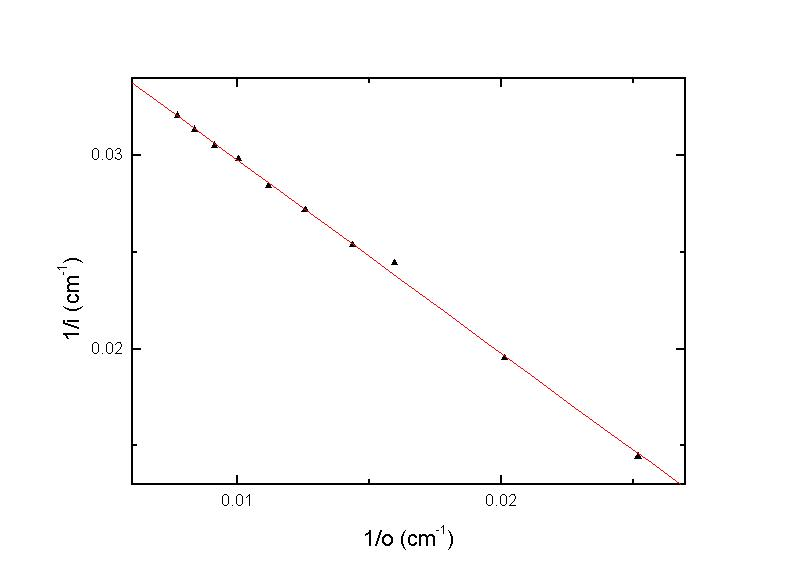
\includegraphics[scale=0.5]{figuras/lc.jpg}
  %\caption{\footnotesize $1/i$ relaciona-se linearmente com $1/o$, sendo o coeficiente linear o inverso
	%da dist�ncia focal.} 
%\end{figure}  

	Conv�m comentar que os limites superior e inferior dos dados coletados foram determinados,
respectivamente, pelo suporte da lente, que j� n�o era grande o bastante para focalizar a imagem, e pela 
amplifica��o, que j� n�o cabia no anteparo.


	Com rela��o � amplifica��o linear, verificamos uma concord�ncia muito boa entre as equa��es

\begin{minipage}[c]{0.46\textwidth}
  $$
  m = -{i\over o} 
  $$
\end{minipage} 
e
\begin{minipage}[c]{0.46\textwidth} 
  $$
  m = {h_i\over h_o}\mathrm{,}
  $$ 
\end{minipage}

	onde $h_i$ e $h_o$ s�o as dimens�es verticais da imagem e do objeto, respectivamente. Como n�o
h� nenhum ajuste ou an�lise mais aprofundada a se fazer com rela��o a este ponto conv�m apresentar os
dados obtidos tanto por uma quanto pela outra equa��o:

\begin{table}[htbp]
  \centering
  \label{tab:amplifica��o linear} 
  \begin{tabular}{c|c}
  $m =h_i/h_o $		&	$m = -i/o$	 	\\
  \hline
  1,70			&	1,74			\\
  1,02			&	1,03			\\
  0,72			&	0,65			\\
  0,55			&	0,57			\\
  0,45			&	0,46			\\
  0,38			&	0,39			\\
  0,34			&	0,34			\\
  0,30			&	0,30			\\
  0,28			&	0,27			\\
  0,26			&	0,24			\\
  \hline
  \end{tabular} 
  \caption{\footnotesize Compara��o entre as amplifica��es lineares obtidas por cada uma das equa��es
	$m=-i/o$ e $m=h_i/h_o$ aplicadas aos dados colhidos no experimento.}
\end{table} 

	
    
 







  \subsection{Lentes divergentes}\label{sec:ld} 
    	No caso das lentes divergentes o processo � significativamente mais complicado, uma vez que este
tipo de lente forma imagens virtuais e, portanto, imposs�veis de se projetar. O ``truque'' para resolver
este problema � associar uma lente convergente cuja dist�ncia focal conhecemos. Neste caso temos duas
op��es:

\begin{itemize}
\item Organizamos em seq��ncia o {\bf objeto} (fonte luminosa), uma lente {\bf convergente}, uma lente 
	{\bf divergente} e o {\bf anteparo}, ou
\item Alteramos as posi��es das duas lentes para obter a seq��ncia {\bf objeto}, lente {\bf divergente},
	lente {\bf convergente} e {\bf anteparo}.
\end{itemize} 

%\begin{figure}[htb]
  %\centering
  %\label{fig:op��o 1}
  %\includegraphics[scale=0.5]{figuras/Ald1.jpg}
  %\caption{\footnotesize A primeira op��o para se medir a dist�ncia focal de uma lente divergente consiste
	%em projetar uma imagem real, oriunda da lente convergente, na lente divergente que, por sua vez,
	%produz uma imagem virtual do lado {\bf real}, entretanto. Esta pode, ent�o, ser projetada num
	%anteparo e as medidas pertinentes serem feitas.} 
%\end{figure}

	A id�ia da primeira op��o � fazer da {\bf imagem real} da lente {\it convergente} o 
{\bf objeto virtual} da lente divergente. Como este objeto � virtual, localiza-se no lado real da
configura��o (Perceba a origem dos feixes de luz). Ao projet�-lo sobre a lente divergente, esta forma
uma imagem no mesmo lado do objeto. Ou seja, {\bf real}, e n�o mais virtual. Esta obviamente pode ser
projetada no anteparo. 

	Ent�o, na figura 7, o anteparo deve ser colocado na posi��o da {\it imagem 2}.
Poder-se-ia argumentar: ``Mas se colocarmos o anteparo na posi��o da imagem 2 os feixes de luz da
imagem 1 -- objeto da segunda lente -- seriam bloqueados pelo anteparo!''. Isto de fato n�o ocorre
simplesmente porque o processo de forma��o da imagem n�o acontece em passos, como no desenho. Os feixes
atravessam a lente convergente e, em seguida, a lente divergente, formando diretamente a imagem 2. O
desenho acima � apenas uma representa��o do processo. 

%\begin{figure}[htb]
  %\centering
  %\label{fig:op��o 2}
  %\includegraphics[scale=0.5]{figuras/Ald2.jpg}
  %\caption{\footnotesize Alternativamente fazemos com que a imagem virtual da lente divergente, atingida
	%primeiramente pelos feixes de luz, seja o objeto real da lente convergente que, por sua vez,
	%projeta a imagem real num anteparo.} 
%\end{figure} 

	A segunda op��o � ligeiramente diferente: Procuramos utilizar a {\bf imagem virtual} da lente 
divergente como {\bf objeto real} da lente {\it convergente} que, por sua vez, forma outra imagem, 
{\bf real} e projet�vel. O processo aqui � deveras mais compreens�vel que na op��o anterior.

	Verificou-se experimentalmente que a primeira op��o era ruim pois exigia uma proximidade excessiva
entre as duas lentes e o anteparo\footnote{Esta proximidade era exigida pela amplifica��o e pelo ponto de 
forma��o das imagens, que de forma alguma cabiam no anteparo e no suporte das lentes.}, dificultando as 
medidas e reduzindo enormemente a faixa de valores mensur�veis. Assim esta forma foi deixada de lado e 
preferimos utilizar a segunda op��o. Tamb�m por quest�es pr�ticas escolhemos n�o a lente $C36$, a qual j� 
hav�amos determinado a dist�ncia focal, mas a $C5$, cuja dist�ncia focal, sendo menor, permitia uma gama 
maior de possibilidades de medidas.

	O procedimento ent�o � o seguinte: Fixamos as duas lentes e variamos as posi��es da fonte 
(objeto 1) e do anteparo (imagem 2), medindo a posi��o de cada um desses componentes. Com isso somos 
capazes de medir $(o_1,\sigma_{o_1})$ e $(i_2,\sigma_{i_2})$. A partir de $o_1$, e conhecendo a dist�ncia
focal da lente convergente $C5$ ($14,40\,\mathrm{cm}$), podemos calcular a posi��o do objeto real desta
lente:
	$$
	{1\over o_2} = {1\over f_c}-{1\over i_2},
	$$
	
	que � a imagem da primeira lente (divergente -- $D25$). Na �ltima express�o denotamos a dist�ncia
focal por $f_c$ para identificar que se trata da lente {\bf c}onvergente. Significado an�logo t�m $f_d$.
Al�m disso, $o_2,\,i_2,\,f_c>0$, o que caracteriza a lente como convergente.

	Uma vez que acabamos de encontrar a posi��o da imagem da primeira lente (Objeto da segunda) e medimos
a posi��o do primeiro objeto, podemos determinar a dist�ncia focal da lente divergente.
	$$
	{1\over f_d} = {1\over i_1}+{1\over o_1}
	$$

	A partir daqui o processo � id�ntico ao da lente convergente, pois j� determinamos $(o,\sigma_o)$ e
$(i,\sigma_i)$: $y=1/i$ e $x=1/o$. Ressalva-se, entretanto, que como a lente � divergente, $i,f_d<0$ e $o>0$.
Encontramos $y=-0,111(7)-1,61(3)x$. Ent�o
	$$
	f_d = {1\over-0,111} \Rightarrow f_d = -9,0(6)\,\mathrm{cm}
	$$

%\begin{figure}[htb]
  %\centering
  %\label{fig:lentes divergentes}
  %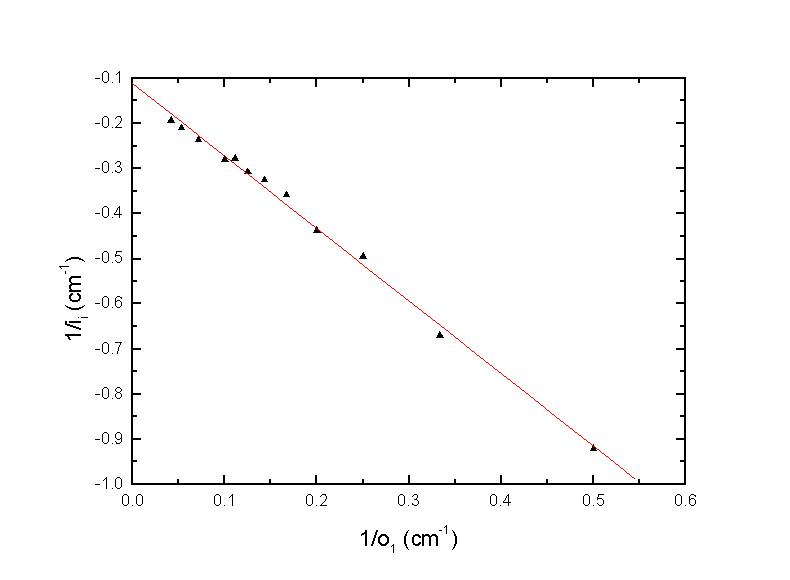
\includegraphics[scale=0.5]{figuras/ld.jpg}
  %\caption{\footnotesize Resultados obtidos na determina��o da dist�ncia focal de uma lente divergente.}  
%\end{figure} 

	Aqui, entretanto, percebemos que o coeficiente linear est� bem longe de ser $1$. Isto indica um 
erro sistem�tico no experimento, que cresce conforme a dist�ncia entre os componentes do experimento 
diminui. Isto n�o � de espantar pois, embora melhor que a op��o 1, este processo de medida tamb�m
n�o foi o que se poderia dizer ``uma beleza'', principalmente quando o anteparo localizava-se
pr�ximo �s lentes, dificultando o acesso visual. Bastante provavelmente podemos incluir a� tamb�m o
cansa�o visual decorrente da extenuante tarefa de procurar a melhor focaliza��o da imagem.  
 





 
  \subsection{Amplifica��o angular da lupa}\label{sec:lupa}  
    	A amplifica��o angular da lupa pode ser determinada simplesmente visualizando-se uma escala
a certa dist�ncia atrav�s da lupa. Escolhendo a imagem de forma a ficar focalizada no olho, ou seja,
simplesmente escolhendo a melhor imagem para os nossos olhos, automaticamente estamos determinando a 
posi��o da imagem. Percorremos este processo para cada um dos olhos de cada um dos elementos do grupo
(2 no caso). Vejamos um caso: Olho direito do Rog�rio: O Rog�rio posicionou-se e a lupa de forma
a ver uma escala em cent�metros verticalmente fixada na parede atrav�s da lupa. O Ivan, por sua vez,
mediu as dist�ncias da parede � lupa e ao olho direito do Rog�rio, encontrando, respectivamente,
$11,5\,\mathrm{cm}$ e $31,5\,\mathrm{cm}$. O Rog�rio disse que enxergou a refer�ncia $0\,\mathrm{cm}$
na parte inferior do di�metro da lupa e $3,5\,\mathrm{cm}$ na parte superior. Como j� hav�amos medido
o di�metro da lupa e encontrado $\phi = 4,4\,\mathrm{cm}$, isto significa que um objeto de 
$3,5\,\mathrm{cm}$ de
altura passou a ser enxergado pelo olho direito do Rog�rio como tendo $4,4\,\mathrm{cm}$ de altura.

	O �ngulo sob o qual o Rog�rio enxergou o {\bf objeto} � simplesmente a altura do objeto dividida
pela dist�ncia dos olhos at� a parede:
	$$
	\tan\theta_o={h_o\over D_o}={3,5\over31,5}=0,\dot{1} \Rightarrow \theta_o=6,34^{\mathrm{o}}
	$$

	e o �ngulo de visada da {\bf imagem} �
	$$
	\tan\theta_i={h_i\over D_i}={4,4\over31,5-11,5}=0,22 \Rightarrow \theta_i=12,41^{\mathrm{o}} 
	$$

	Portanto a amplifica��o angular $m_\theta$ �
	$$
	m_\theta = {\theta_i\over\theta_o}={12,41\over6,34}=1,96
	$$

	A amplifica��o angular m�xima prevista para o Rog�rio (E tamb�m para o Ivan, j� que ambos
tem ponto pr�ximo de $11\,\mathrm{cm}$) �
	$$
	M_\theta = {11\over f}+1\,\,\,\,\,\mathrm{[f]=cm}
	$$

	onde $f$ � o foco da lupa. Utilizamos a lente $C5$ ($f=14,40\,\mathrm{cm}$) e, portanto
$M=1,76$. Mas este valor � razoavelmente menor que a amplifica��o encontrada. Isto n�o importa muito
pois o procedimento de medida � extremamente incerto, j� que, primeiro, fizemos o experimento de p�;
Segundo, seguramos a lente e a r�gua que utilizamos para encontrar as dist�ncias com as pr�prias m�os; E
por fim, h� muita margem para paralaxes na medida das dist�ncias, isso sem falar que n�o levamos em conta
o di�metro do globo ocular. Se assim o fizermos, aumentando em aproximadamene $8\,\mathrm{cm}$ as
duas dist�ncias, encontraremos $m_\theta=1,76$. Ou seja, apesar de tudo os resultados s�o bons.

	Abaixo apresentamos o resultado para cada um dos componentes do grupo.

\begin{table}[htbp]
\begin{minipage}[b]{0.46\textwidth} 
  \centering
  \begin{tabular}{cc|cc}
  \multicolumn{4}{c}{Ivan} 							\\
  \hline												
  \multicolumn{2}{c}{Olho direito} & \multicolumn{2}{c}{Olho esquerdo} 		\\
  \hline									
  $2,19$	&	$1,91^*$	&	$1,84$	&	$1,68^*$ 	\\
  \hline									
  \end{tabular} 
\end{minipage}
\hfill
\begin{minipage}[b]{0.46\textwidth}
  \centering
  \begin{tabular}{cc|cc} 							
  \multicolumn{4}{c}{Rog�rio} 							\\	
  \hline									
  \multicolumn{2}{c}{Olho direito} & \multicolumn{2}{c}{Olho esquerdo} 		\\
  \hline									
  $1,96$	&	$1,76^*$	&	$1,24$	&	$1,12^*$	\\
  \hline				
  \end{tabular}
\end{minipage} 
  \caption{\footnotesize Amplifica��o angular de uma lupa com dist�ncia focal $14,40\,\mathrm{cm}$ a
	v�rias dist�ncias para cada um dos olhos de cada um dos componentes de grupo. Os valores com
	asterisco (*) levam em considera��o o di�metro do globo ocular, tomado como $8\,\mathrm{cm}$.} 
\end{table} 



 
  \subsection{Efeito lupa num orif�cio}\label{sec:orificio}  
    	Um orif�cio pode ser utilizado como lupa se for suficientemente pequeno quandocomparado com os 
objetos que se pretende observar. O princ�pio � bastante simples e n�o passa de semelhan�a de 
tri�ngulos. Observe a figura 10,

%\begin{figure}[htb]
  %\centering
  %\label{fig:orif�cio}
  %\includegraphics[scale=0.5]{figuras/orificio1.jpg}
  %\caption{\footnotesize Um orif�cio funciona como lupa quando for suficientemente pequeno.} 
%\end{figure} 

	Tiramos imediatamente que
	$$
	{h_o\over D_o}={h_i\over D_i} \Rightarrow h_i = {D_i\over D_o}h_o
	$$

	e, se $D_i>D_o$, ent�o � claro que $h_i>h_o$, significando uma amplia��o linear. Em verdade,
note ainda que a express�o acima pode ser escrita como
	$$
	{h_i\over h_o}={D_i\over D_o}
	$$

	que � exatamente a express�o da amplifica��o linear, a menos do sinal negativo inclu�do 
simplesmente por quest�o de conven��o.

	Outro aspecto interessante de se notar � que analisando cuidadosamente o movimento dos
objetos atrav�s do orif�cio percebemos que a velocidade com que se movem, no sentido contr�rio, � 
aparentemente maior que a velocidade com que se move o orif�cio. Isto se deve ao fato de que
inconscientemente movemo-nos no sentido do orif�cio um pouco mais r�pido, procurando focalizar um
ponto do objeto atr�s do orif�cio. Veja a figura 11,

%\begin{figure}[htb]
  %\centering
  %\label{fig:orif�cio movimento}
  %\includegraphics[scale=0.5]{figuras/orificio2.jpg}
  %\caption{\footnotesize O movimento aparentemente estranho dos objetos quando observados atrav�s de
	%um pequeno orif�cio.} 
%\end{figure} 

	� f�cil ver que
	$$
	{d\over D}={s_0\over s_A} \Rightarrow {d/t\over D/t}={s_0\over s_A} \Rightarrow {v_0\over v_A}=
		{s_0\over s_A} \Rightarrow v_A={s_A\over s_0}v_0
	$$

	e, portanto, se $s_A>s_0$, veremos os objetos atrav�s do orif�cio moverem-se mais rapidamente que
movimentamos o orif�cio. Este efeito � id�ntico �quela situa��o em que, por exemplo, estando pr�ximo
a um poste e nos movimentando procuramos observar um carro, mais r�pido e mais longe do poste, exatamente 
atr�s deste. Muitas vezes ocorre de  n�o conseguirmos ver o carro durante um certo per�odo de tempo pois,
embora estejamos movendo-nos a velocidades diferentes, a linha que nos liga passa sempre pelo poste.




 
  \subsection{Polariza��o do laser He--Ne}\label{sec:HeNe}
    	O laser de He--Ne utilizado na experi�ncia n�o � polarizado. Al�m disso, n�o existe homogeneidade
dos campos el�tricos perpendiculares � dire��o de propaga��o. Isto � suficiente para impedir-nos de
utiliz�-lo como fonte n�o polarizada e/ou polarizada. Mais que isso: Como pretendemos utilizar algum
plano de polariza��o para os experimentos seguintes, decorre a necessidade de um polar�ide. 

	Entretanto, o polar�ide por si s� n�o resolve o problema pois detectamos que mesmo a esperada 
onda polarizada ap�s o polar�ide oscila temporalmente em intensidade, indicando-nos que n�o s� o laser
n�o � polarizado como tamb�m varia com o tempo. Este tempo foi avaliado em $7$ minutos aproximadamente. 

%\begin{figure}[htb]
  %\centering
  %\includegraphics[scale=0.5]{figuras/HeNe.jpg}
  %\caption{\footnotesize Arranjo esquem�tico utilizado para a verifica��o do comportamento ``quase'' 
	%polarizado 
	%do laser. Embora n�o haja polariza��o plana do feixe, os diversos planos de oscila��o do campo 
	%el�trico mudam com o tempo, caracterizando uma luz bastante ruim de se trabalhar quando 
	%necessitamos de luz polarizada.} 
%\end{figure} 

	Surge ent�o a necessidade de procurarmos uma fonte mais est�vel. Por isso o laser foi utilizado
apenas para determinarmos o �ngulo de Brewster, cujas medidas n�o s�o afetadas pela mudan�a dos planos
de oscila��o da onda. Para os outros experimentos -- Lei de Malus (sess�o \ref{sec:malus}) e
coeficientes de reflex�o (sess�o \ref{sec:coeficientes}) -- utilizamos uma l�mpada 
incandescente de tungst�nio, cuja emiss�o � uniforme -- ou quase -- em todas as dire��es.
 
  \subsection{�ngulo de Brewster}\label{sec:brewster} 
    	O �ngulo de Brewster para o lucite foi obtido organizando nossos aparelhos da forma ilustrada
na figura 13:

%\begin{figure}[htb]
  %\centering
  %\label{fig:brewster}
  %\includegraphics[scale=0.5]{figuras/Abrewster.jpg}
  %\caption{\footnotesize Arranjo experimental que permitiu a medi��o do �ngulo de Brewster para o lucite.}
%\end{figure} 

	O que se fez foi variar o �ngulo de incid�ncia do laser sobre o lucite atrav�s do goni�metro e 
procurar o feixe refletido pela primeira superf�cie cuja intensidade fosse zero ou a menor poss�vel. Na 
maioria dos casos encontrava-se uma intensidade n�o nula mas bastante fraca. Isto ocorre devido �s 
imperfei��es na superf�cie do lucite\footnote{Possivelmente devido tamb�m � oleosidade das m�os dos
elementos do grupo que agregava-se durante o manuseio do bloco de lucite.}.

	Deste modo, fizemos o experimento um total de $6$ vezes seguidas, retornando-se sempre antes de
cada medida � posi��o de incid�ncia $0^{\mathrm{o}}$ (normal � superf�cie do lucite). Isto � necess�rio 
pois o goni�metro n�o � um equipamento perfeito: Procur�vamos a posi��o de incid�ncia normal n�o lendo
a escala do goni�metro, mas sim fazendo com que o laser refletido fosse direcionado para a fonte que o
originou, garantindo a incid�ncia normal. Mas, quando isto era feito, notava-se que o goni�metro indicava
uma incid�ncia entre $+1^{\mathrm{o}}$ e $-1^{\mathrm{o}}$, inclusive. Esta flutua��o foi levada em 
considera��o nos c�lculos, adicionando-se ou subtarindo-se este pequeno erro ao valor de �ngulo de
Brewster encontrado. Por exemplo: Numa das medidas encontramos que o feixe refletido tinha sua intensidade
m�nima (�ngulo de Brewster) em $56^{\mathrm{o}}$ e o erro inicial era de $1^{\mathrm{o}}$. Ent�o o
�ngulo efetivamente encontrado foi $55^{\mathrm{o}}$. Este tipo de flutua��o deve-se principalmente ao
afrouxamento existente entre as pe�as m�veis que constitui o goni�metro e � m�scara\footnote{A m�scara
de alinhamento � um pequeno desn�vel existente entre um semi-c�rculo e outro do goni�metro, que permite
posicionarmos a superf�cie do lucite exatamente no centro de rota��o do goni�metro.} de alinhamento do
bloco de lucite.

	Encontramos, ent�o, para o �ngulo de Brewster, $\theta_B=54,25(28)^{\mathrm{o}}$. A incerteza
foi calculada como a incerteza da m�dia das seis medidas efetuadas: $\sigma_{\theta_B}=\sigma/\sqrt{6}$,
com $\sigma$ o desvio padr�o da distribui��o.

	Considerando o �ndice de refra��o do ar igual a unidade, conclu�mos que o �ndice de refra��o $n$ do
lucite e o �ngulo de Brewster relacionam-se aproximadamente por
	$$
	\tan\theta_B\cong n
	$$

	Por conseguinte, $n=1,389(14)$.
   











 
  \subsection{Lei de Malus}\label{sec:malus} 
    	Como foi visto na introdu��o te�rica, a lei de Malus relaciona a intensidade da luz polarizada
com o �ngulo $\theta$ de inclina��o da malha do polar�ide (e, portanto, o plano de polariza��o daquele
polar�ide). Para fazermos esta medida precisamos de
dois polar�ides: O primeiro para polarizar num plano conveniente a luz proveniente da fonte n�o 
polarizada e o segundo para variarmos o plano da malha (fig.14).

%\begin{figure}[htb]
  %\centering
  %\label{fig:malus 1} 
  %\includegraphics[scale=0.5]{figuras/malus1.jpg}
  %\caption{\footnotesize Arranjo experimental utilizado na verifica��o da Lei de Malus. O primeiro
	%polar�ide garante que a luz incidente sobre o segundo � polarizada.}
%\end{figure} 

	As medidas foram feitas desde $\theta=0^{\mathrm{o}}$ at� $\theta=180^{\mathrm{o}}$, tomando o
cuidado de se verificar as intensidades para $\theta=0^{\mathrm{o}}$ e $\theta=90^{\mathrm{o}}$ antes de
cada medida. Este procedimento � necess�rio pois a fonte luminosa de tungst�nio ainda sim n�o �
necessariamente perfeitamente homog�nea em sua emiss�o, e isto pode causar alguma flutua��o na medida,
o que de fato ocorreu, como pode ser visto na figura 15:

%\begin{figure}[htb]
  %\centering
  %\label{fig:malus 2}
  %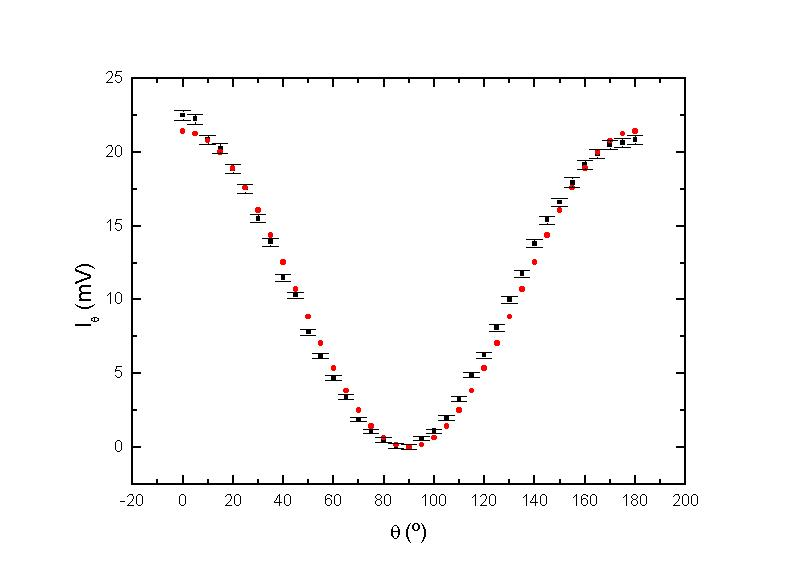
\includegraphics[scale=0.5]{figuras/malus2.tex}
  %\caption{\footnotesize A intensidade m�xima do feixe emergente do segundo polar�ide flutua um
	%pouco, como se pode verificar. Isto se deve �s imperfei��es de emiss�o da luz incandescente.
	%Os valores em vermelho s�o os esperados teoricamente, considerando a intensidade m�xima como
	%a m�dia da flutua��o encontrada.} 
%\end{figure}

	Uma alternativa para resolver este problema � usar intensidades normalizadas pela intensidade
m�xima. Neste caso o que se faz � tomar uma medida de $I_\theta$, subtair $I_f$ para aquele caso  e 
divid�-la 
por $I_0$. Isto feito chegamos � figura 16:

%\begin{figure}[htb]
  %\centering
  %\label{fig:malus 3}
  %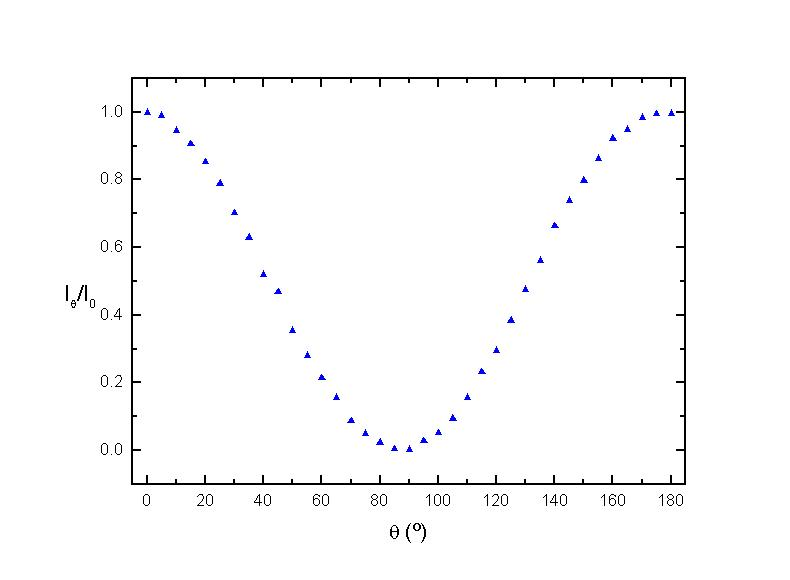
\includegraphics[scale=0.5]{figuras/malus3.jpg}
  %\caption{\footnotesize O mesmo resultado da figura \ref{fig:malus 2} normalizando os valores das 
	%intensidades e excluindo a radia��o de fundo $I_f$.} 
%\end{figure} 

	Pela teoria de Malus, a intensidade $I_\theta$ do feixe polarizado deve variar conforme
	$$
	I_\theta = I_0 \cos^2\theta +I_f,
	$$  

	onde $I_0$ � a intensidade para $\theta=0^{\mathrm{o}}$ e $I_f$ a intensidade para 
$\theta=90^{\mathrm{o}}$ (radia��o de fundo pois nesta situa��o o polar�ide bloqueia totalmente a luz
incidente).

	Podemos ent�o normalizar esta equa��o fazendo $x=\cos^2\theta$ e $y=I_\theta$. Isto posto plotamos
a figura 17:

%\begin{figure}[htb]
  %\centering
  %\label{fig:malus 4}
  %\includegaphics[scale=0.5]{figuras/malus4.jpg}
  %\caption{\footnotesize Lineariza��o da lei de Malus, cujo objetivo � determinarmos experimentalmente os
	%valores de $I_0$ e $I_f$.}
%\end{figure}

	E conclu�mos que
	$$
	I_\theta = 21,4(3)\cos^2\theta+0,11(15)
	$$

	As intensidades na express�o anterior s�o dadas, na realidade, em $\mathrm{mV}$, a tens�o sobre
o resistor de carga do circuito do fotodiodo utilizado no experimento (figura 18).

%\begin{figure}[htb]
  %\centering
  %\label{fig:foto diotod}
  %\includegraphics[scale=0.5]{figuras/fotodiodo.jpg}
  %\caption{\footnotesize Fotodiodo utilizado para medir as intensidades luminosas e sua rela��o entre
	%corrente, em $m\mathrm{A}$ de coletor e intensidade luminosa, em $\mathrm{mW/cm^2}$.}
%\end{figure} 

	 

	
 
  \subsection{Coeficientes de reflex�o}\label{sec:coeficientes}  
    	A intensidade do feixe refletido por uma superf�cie diel�trica depende do �ngulo de incid�ncia.
De fato, vimos anteriormente que para um determinado �ngulo -- o  de Brewster -- a intensidade do
feixe polarizado paralelamente � superf�cie do diel�trico � zero. O comportamento da intensidade de uma
luz n�o polarizada incidente numa tal superf�cie � um pouco dif�cil de medir, mas � bastante mais f�cil
determinar separadamente as intensidades dos feixes polarizados paralela e perpendicularmente � 
superf�cie do diel�trico para, em seguida, calcularmos a raz�o $r=I_\parallel/I_\perp$, que d� uma boa
no��o do comportamento.

	O que fizemos ent�o foi disponibilizar o arranjo da figura \ref{fig:coeficiente} e medirmos
as intensidades para $\phi=0^{\mathrm{o}}$ e $\phi=90^{\mathrm{o}}$\footnote{Note que, diferentemente
do caso da lei de Malus, n�o fazemos uma sele��o pr�via do plano de incid�ncia desejado.}.

%\begin{figure}[htb]
  %\centering
  %\label{fig:coeficiente} 
  %\includegraphics[scale=0.5]{figuras/Acoeficientes.jpg} 
  %\caption{\footnotesize Arranjo experimental utilizado na verifica��o dos coeficientes de refles�o. O
	%filtro � utilizado para bloquear os raios infravermelhos, ignorados pelo polar�ide mas n�o pelo
	%fotodiodo.}
%\end{figure}

	Teoricamente o que se espera �
	$$
	r={R_\parallel\over R_\perp}={{\tan^2(\hat i-\hat t)\over\tan^2(\hat i+\hat t)}\over
					{\sin^2(\hat i-\hat t)\over\sin^2(\hat i+\hat t)}}=
					{\cos^2(\hat i+\hat t)\over\cos^2(\hat i-\hat t)}
	$$

	onde $\hat i$ e $\hat t$ s�o, respectivamente, os �ngulos de incid�ncia e refra��o (transmiss�o). 
Variamos $\hat i$ desde $15^{\mathrm{o}}$, o m�nimo permitido pelo goni�metro, at� $70^{\mathrm{o}}$,
onde o feixe incidente passava a influenciar drasticamente na leitura do fotodiodo. Isto porque a fonte
de luz utilizada era suficientemente extensa para possuir raios que incidiam diretamente sobre o fotodiodo
sem serem refletidos no lucite.

	O resultado obtido, comparado com o toricamente esperado � apresentado na figura 19.

%\begin{figure}[htb]
  %\centering
  %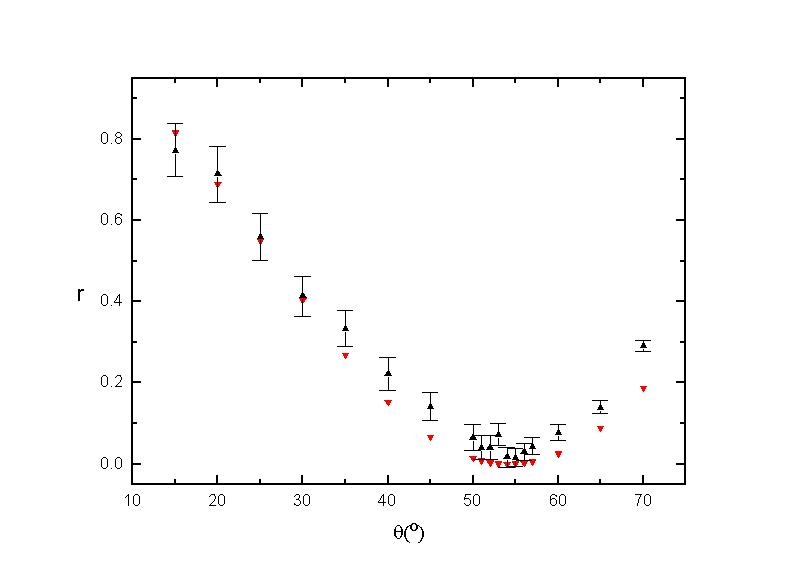
\includegraphics[scale=0.5]{figuras/coeficientes.jpg}
  %\caption{\footnotesize O comportamento da raz�o $r$ entre as intensidades dos feixes polarizados paralela 
	%e perpendicularmente � superf�cie do lucite em compara��o com o esperado teoricamente. Note o
	%�ngulo de Brewster a aproximadamente $\hat i = 54^{\mathrm{o}}$.}
%\end{figure} 

 
  \subsection{Birrefring�ncia e fotoelasticidade}\label{sec:birrefring�ncia}  
    	Nossa experi�ncia neste t�tulo limitou-se a divertirmo-nos observando s�lidos anisotr�picos
que respondiam diferentemente � refra��o face uma press�o ou tens�o sofrida. A figura 20 mostra dois
exemplos de birrefring�ncia parecidos com aqueles que vimos durante o experimento.  
\section{Conclus�es}
  	Todos os experimentos tiveram concord�ncia muito boa com a teoria, exceto talvez o caso da
lente divergente que, como comentamos, apresentou um erro sistem�tico bastante elevado em compara��o
com todos os outros resultados obtidos. 
	Mas existe um ponto que n�o foi sequer inclu�do no seu respectivo local pois apresentou 
resultados absurdos. Trata-se da determina��o do �ndice de refra��o da lente a partir da f�rmula do
fabricante de lentes:
	$$
	{1\over f}=(n-1)[{1\over R_2}-{1\over R_1}]+{(n-1)^2\over n}{t\over R_1R_2}
	$$

	em primeira aproxima��o desconsideramos a segunda parcela e utilizamos
	$$
	{1\over f}=(n-1)[{1\over R_2}-{1\over R_1}]
	$$

	A dist�ncia focal, da lente convergente $C36$ por exemplo, foi determinada na sess�o \ref{sec:lc}:
$f=25,14(3)\,\mathrm{cm}$ e os raios $R_1$ e $R_2$ medidos atrav�s de um pequeno aparelho chamado 
rel�gio, que relacionava sua escala $x$ com o raio de curvatura da lente atrav�s da express�o
	$$
	{1\over R}=1,92\cdot x+0,4\,\,\,\,\,\,\mathrm{[R]=m}
	$$

	Para este caso espec�fico medimos $x=1,75$ e $x=1,875$, que correspondem respectivamente a
$R_1=26,60\,\mathrm{cm}$ e $R_2=25,00\,\mathrm{cm}$. Mas estes valores s�o muito pr�ximos da dist�ncia
focal encontrada. Este � o primeiro ponto estranho. Se insistirmos nestes valores e procurarmos calcular
os �ndices de refra��o, encontramos $n=17,53$, muito alto!\footnote{O valor mais pr�ximo que pudemos obter
atrav�s de \cite[p�g.12-42]{handbook} foi o do Tantalato de pot�ssio ($\mathrm{KTaO_3}$), e subst�ncias
com este �ndice eram muito raras!} Este � o segundo ponto estranho. Se tentarmos
resolver o problema lembrando dos velhos tempos de col�gio onde $R=2f$ e recalcularmos o �ndice, ainda
assim encontramos $n=34,06$, ainda mais absurdo! Segue abaixo a tabela de �ndices de refra��o encontrados
para cada uma das duas lentes convergentes:

\begin{table}[htbp]
  \centering
  \begin{tabular}{cc}
  \hline
  Lente		&	$n$			 	\\
  \hline						
  C36		&	17,53				\\
  C5		&	58,28				\\
  \hline
  \end{tabular}
\end{table}    

	O �ndice de refra��o da lente divergente n�o foi poss�vel medir pois $R_1=R_2=8,22\,\mathrm{cm}$ e,
consequentemente, o primeiro termo anula-se, exigindo a inclus�o do segundo que, por sua vez, exigia a
espessura da lente, que n�o foi medida, por motivos desconhecidos.

	Finalmente repetimos: A despeito deste ponto, todos os outros experimentos foram bem sucedidos.


 
\begin{thebibliography}{9}
  \bibitem{griffiths} D.J.Griffiths, {\it Introduction to eletrodynamics}, third edition, Prentice Hall,
			New Jersey, 1999.
\bibitem{alex}	    A.B. Meyknecht, E.E. Alonso, J.P. Machado, {\it Lentes e
polariza��o da luz}, relat�rio de f�sica experimental IV, IFUSP, 1999. 	
\bibitem{handbook}  D.R. Lide, {\it Handbook of Chemistry and Physics}, $73^{\mathrm{a}}$ed., 1992-1993
 
\end{thebibliography}

\end{document}
 


